\textbf{1. Input data.} The physical parameters specified for the closed-closed acoustic tube are
\[
\boxed{L=0.500\,\mathrm{m},\qquad c=340\,\mathrm{m/s},\qquad \rho=1.2\,\mathrm{kg/m}^3,\qquad N=5}\qquad\text{(B.4.1)}
\]
The associated medium properties are the acoustic bulk modulus and the characteristic acoustic impedance.
\[
K=\rho c^2=1.2\times(340)^2\,\mathrm{Pa}\approx138.7\,\mathrm{kPa},
\qquad
Z=\rho c=1.2\times 340\,\mathrm{Pa\cdot s/m}=408\,\mathrm{rayl}.
\]

\textbf{2. Modal vibration characteristics.} Using the analytical relations derived in Problem B.3, the modal characteristics for modes $j=1,2,3,4,5$ are evaluated as follows:
\par\smallskip\noindent
\textbf{(a) Eigenvalues $z_j$:}
\[
\boxed{z_j=j\pi\quad\Longrightarrow\quad z_1=\pi,\; z_2=2\pi,\; z_3=3\pi,\; z_4=4\pi,\; z_5=5\pi}\qquad\text{(B.4.2.a)}
\]
\textbf{(b) Wavenumbers $\gamma_j$:}
\[
\boxed{\gamma_j=\frac{z_j}{L}=\frac{j\pi}{0.500}\,\mathrm{rad/m}\approx 6.28\,j\,\mathrm{rad/m}}\qquad\text{(B.4.2.b)}
\]
\textbf{(c) Natural circular frequencies $\omega_j$:} Since $c/L=340/0.500=680\,\mathrm{s}^{-1}$,
\[
\boxed{\omega_j=\gamma_j c=\frac{j\pi c}{L}=680\pi j\,\mathrm{rad/s}\approx 2.14\times10^3\,j\,\mathrm{rad/s}}\qquad\text{(B.4.2.c)}
\]
\textbf{(d) Natural frequencies $f_j$ in Hz:}
\[
\boxed{f_j=\frac{\omega_j}{2\pi}=\frac{jc}{2L}=340\,j\,\mathrm{Hz}\quad\Longrightarrow\quad 340,\,680,\,1020,\,1360,\,1700\,\mathrm{Hz}}\qquad\text{(B.4.2.d)}
\]
The corresponding acoustic wavelengths are $\lambda_j=2L/j=1.000/j\,\mathrm{m}$. The complete modal characteristics are summarized in Table~\ref{tab:hw02-b4-modal}.

\begin{table}[H]
\centering
\caption{Modal vibration characteristics of the closed-closed air tube ($L=0.500\,\mathrm{m}$, $c=340\,\mathrm{m/s}$).}
\label{tab:hw02-b4-modal}
\smallskip
\small
\begin{tabular}{@{}cccccc@{}}
\toprule
Mode $j$ & $z_j$ (rad) & $\gamma_j$ (rad/m) & $\omega_j$ (krad/s) & $f_j$ (Hz) & $\lambda_j$ (m) \\
\midrule
1 & $\pi\approx 3.14$ & $6.28$ & $2.14$ & $340$ & $1.000$ \\
2 & $2\pi\approx 6.28$ & $12.57$ & $4.27$ & $680$ & $0.500$ \\
3 & $3\pi\approx 9.42$ & $18.85$ & $6.41$ & $1020$ & $0.333$ \\
4 & $4\pi\approx 12.57$ & $25.1$ & $8.55$ & $1360$ & $0.250$ \\
5 & $5\pi\approx 15.71$ & $31.4$ & $10.68$ & $1700$ & $0.200$ \\
\bottomrule
\end{tabular}
\end{table}

\textbf{3. Displacement modeshapes.} From Problem B.3 (item 20), the displacement modeshapes are
\[
\boxed{U_j(x)=\sin\left(\frac{j\pi x}{L}\right)=\sin\left(\frac{j\pi x}{0.500}\right),\qquad j=1,\ldots,5}\qquad\text{(B.4.3)}
\]
Figure~\ref{fig:hw02-b4-disp} plots the displacement modeshapes for the first five modes across the tube length.

\begin{figure}[H]
\centering
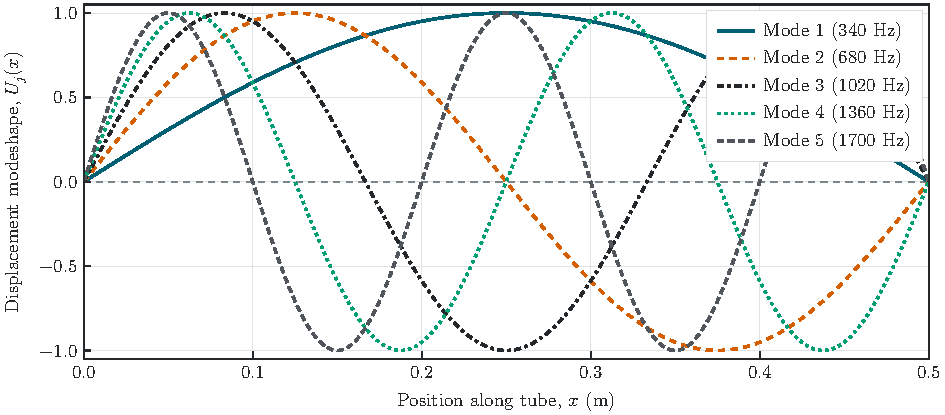
\includegraphics[width=0.96\linewidth]{figures/generated/solutions/B4-displacement.pdf}
\caption{Displacement modeshapes $U_j(x)=\sin(j\pi x/L)$ for modes $j=1,\ldots,5$ in an air tube of length $L=0.500\,\mathrm{m}$ closed at both ends. }
\label{fig:hw02-b4-disp}
\end{figure}

\textbf{4. Discussion of results.}
Both rigid ends are displacement nodes because $U_j(0)=U_j(L)=0$. The fundamental is $f_1=340\,\mathrm{Hz}$, and the higher frequencies are $f_j=jf_1$. The tube therefore supports all integer harmonics.

Each mode fits $j$ half-wavelengths into the tube, so $L=j\lambda_j/2$. For the fundamental, $\lambda_1=2L=1.000\,\mathrm{m}$. Mode $j$ has $j+1$ displacement nodes, including both ends, and $j$ antinodes. Adjacent nodes are separated by $L/j$.


\textbf{5. Graduate work: Normalized pressure modeshapes and comparison.}
From Problem B.3 (item 21), acoustic pressure disturbance is generated by fluid strain, $p(x,t)=-Ku_x(x,t)=-\rho c^2 u_x(x,t)$. For displacement amplitude $a_j>0$ in meters, write $u_j(x,t)=a_jU_j(x)e^{-i\omega_jt}$. Differentiating $U_j(x)=\sin(\gamma_jx)$ gives $U_j'(x)=\gamma_j\cos(\gamma_j x)$, yielding the pressure amplitude
\[
P_j(x)=-\rho c^2a_j\gamma_j\cos\left(\frac{j\pi x}{L}\right)=-\rho c\,\omega_j a_j\cos\left(\frac{j\pi x}{L}\right).
\]
\noindent\begin{minipage}{\linewidth}\color{black}
Normalizing by the peak pressure amplitude $|P_j|_{\max}=\rho c\,\omega_j a_j$ yields the normalized pressure modeshape
\[
\boxed{\bar{P}_j(x)=-\cos\left(\frac{j\pi x}{L}\right)=-\cos\left(\frac{j\pi x}{0.500}\right),\qquad j=1,\ldots,5}\qquad\text{(B.4.5)}
\]
\end{minipage}\par

Figure~\ref{fig:hw02-b4-press} plots the normalized pressure modeshapes for modes $1$ through $5$.

\begin{figure}[H]
\centering
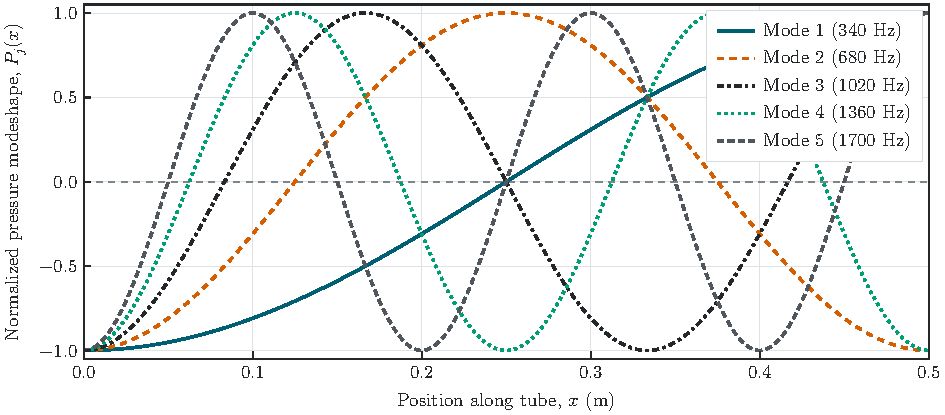
\includegraphics[width=0.96\linewidth]{figures/generated/solutions/B4-pressure.pdf}
\caption{Normalized acoustic pressure modeshapes $\bar{P}_j(x)=-\cos(j\pi x/L)$ for modes $j=1,\ldots,5$ in a closed-closed tube of length $L=0.500\,\mathrm{m}$.}
\label{fig:hw02-b4-press}
\end{figure}

The sine displacement shape and negative-cosine pressure shape differ spatially by a quarter wavelength. Since pressure is proportional to $-U_j'$, displacement antinodes are pressure nodes, and displacement nodes are pressure antinodes.

Both closed ends are pressure antinodes with $|\bar{P}_j|=1$. Mode $j$ has $j$ internal pressure nodes and $j+1$ pressure antinodes, including the two ends. These counts agree with the plotted curves.

\clearpage
\matlabcaption{MATLAB calculations and plots for B.4.}

\lstinputlisting[style=hwmatlab]{matlab/B4.m}
